\section{Removing unreachable blocks}

There could be blocks generated in the previous pass which are \textit{unreachable}, meaning that there is no path from
the \textit{entry block} (whose \code{id} is equal to \code{0}) of the control flow graph to these blocks. The entry
block is reachable by default.

This pass visits the control flow graph, which is a directed graph. If the method body does not contain loops, the graph
is acyclic; otherwise, it contains at least one cycle. A breadth-first search algorithm is used to compute the set of
reachable blocks from the entry block of the control flow graph. After the search is finished, the blocks which are not
contained in the set of reachable blocks are removed from the list of all blocks representing the control flow graph.

An example of this pass is provided in \labelindexref{Figure}{img:remove-unreachable}. The blocks with \code{id}s equal
to \code{2} and \code{5} are unreachable from the entry block, so they get removed. Even though the block with \code{id}
\code{2} is reachable from the block with \code{id} \code{5}, it is not reachable from the entry block (with \code{id}
\code{0}), so it still gets removed.

\begin{figure}[htb]
    \makebox[\linewidth][c]{%
    \begin{subfigure}[b]{.6\textwidth}
        \centering
        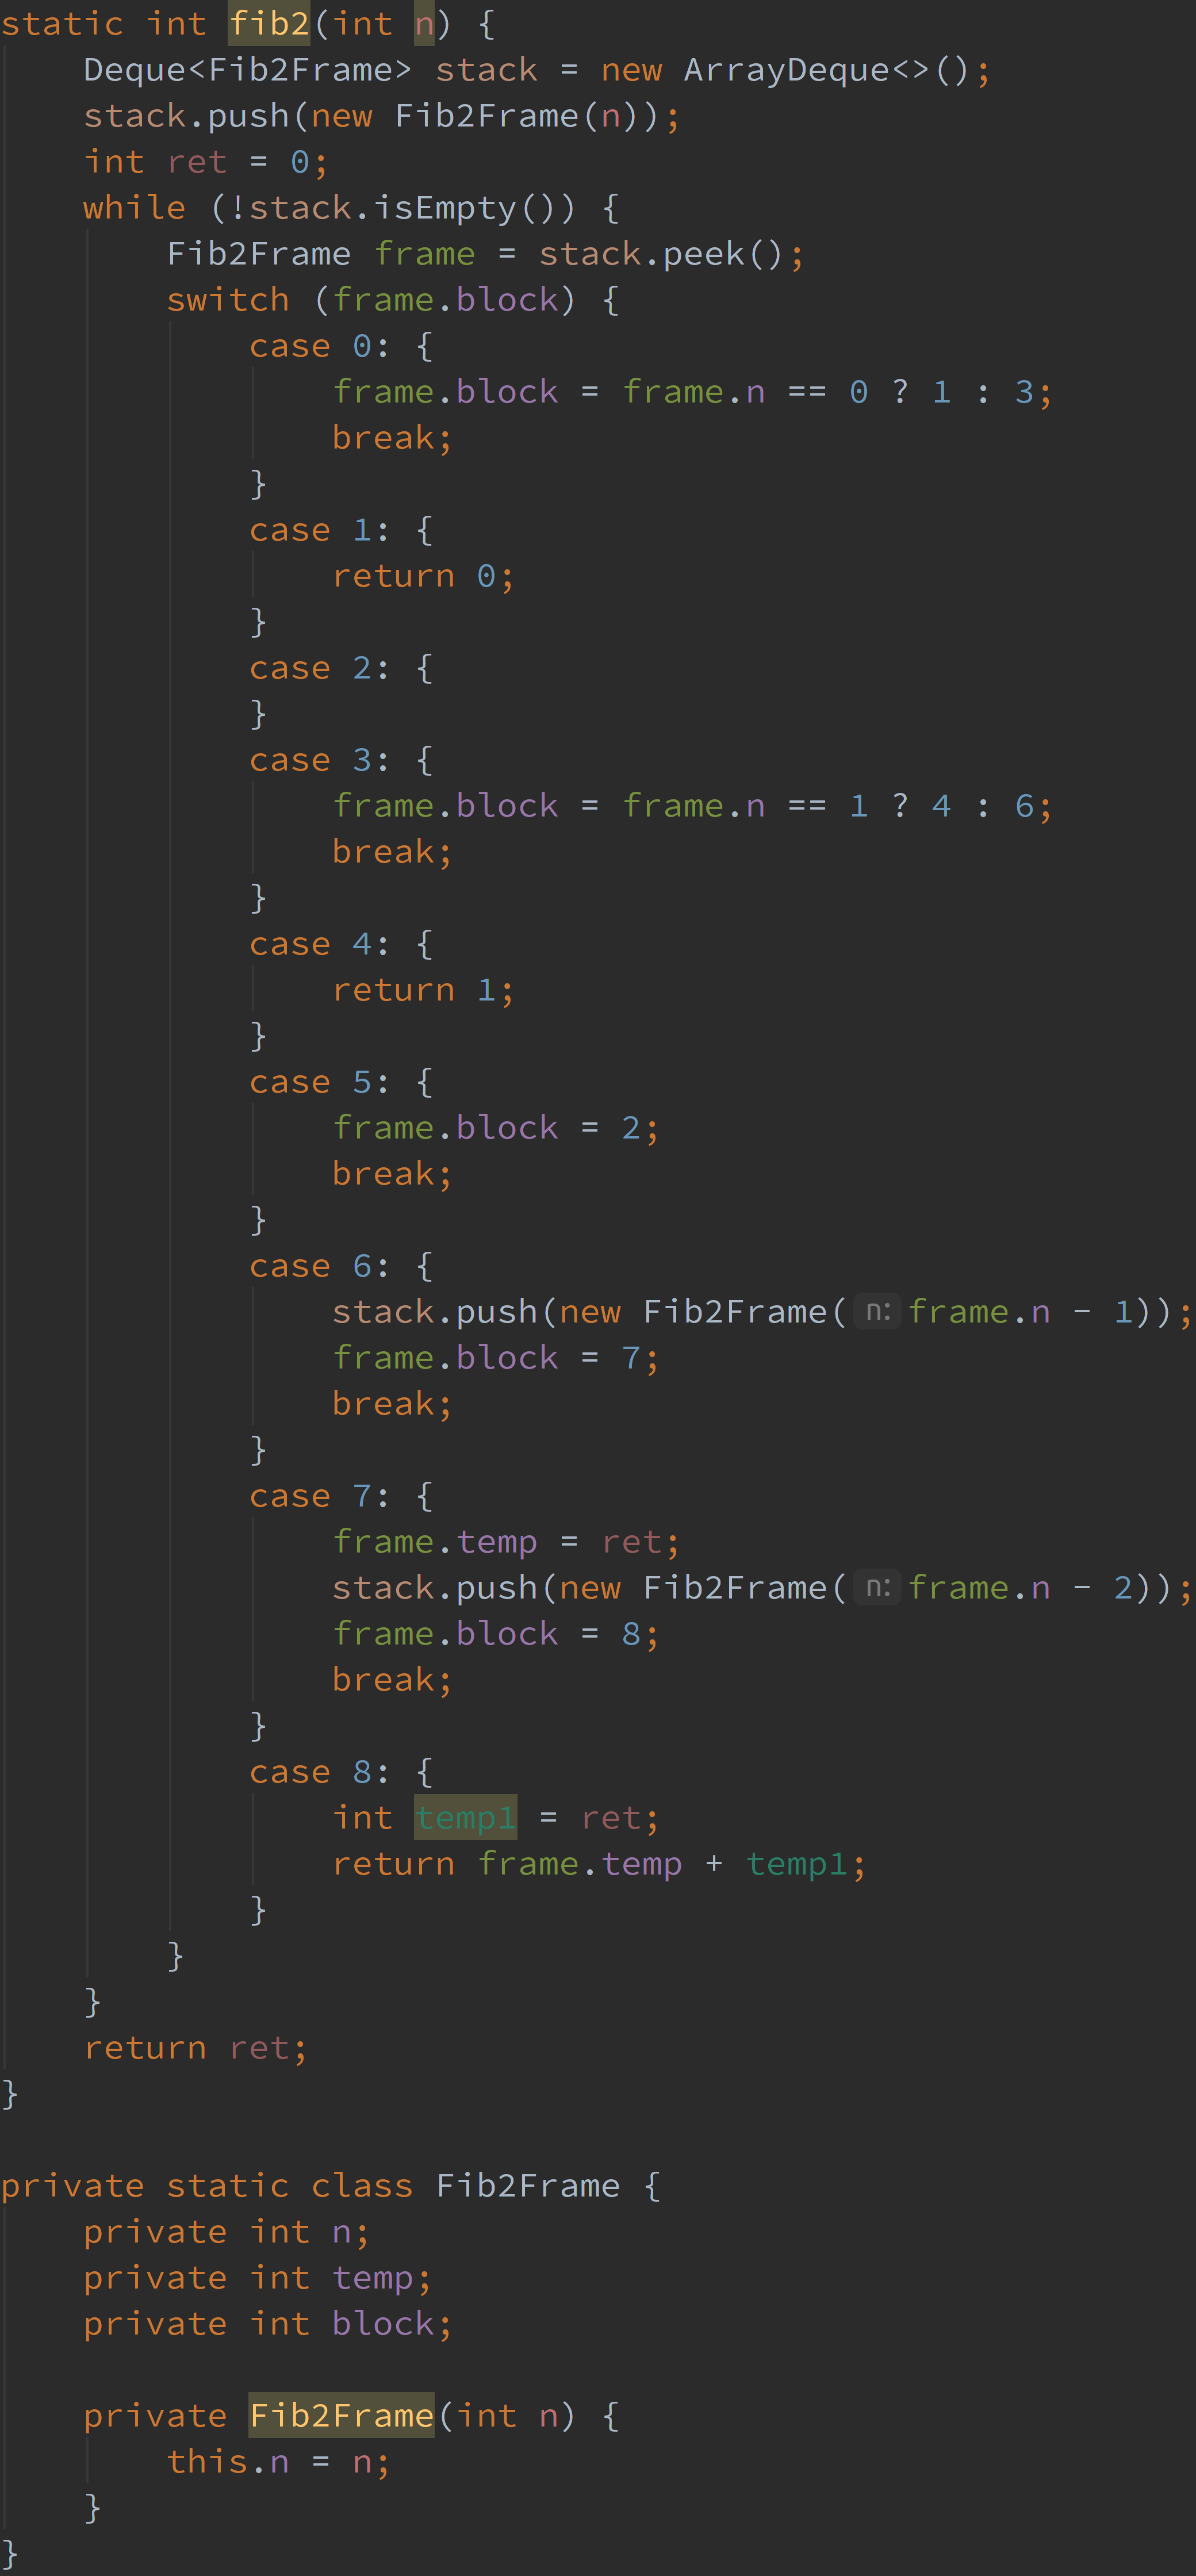
\includegraphics[height=5in]{src/img/blocks-after.png}
        \caption{Before}
    \end{subfigure}%
    \begin{subfigure}[b]{.6\textwidth}
        \centering
        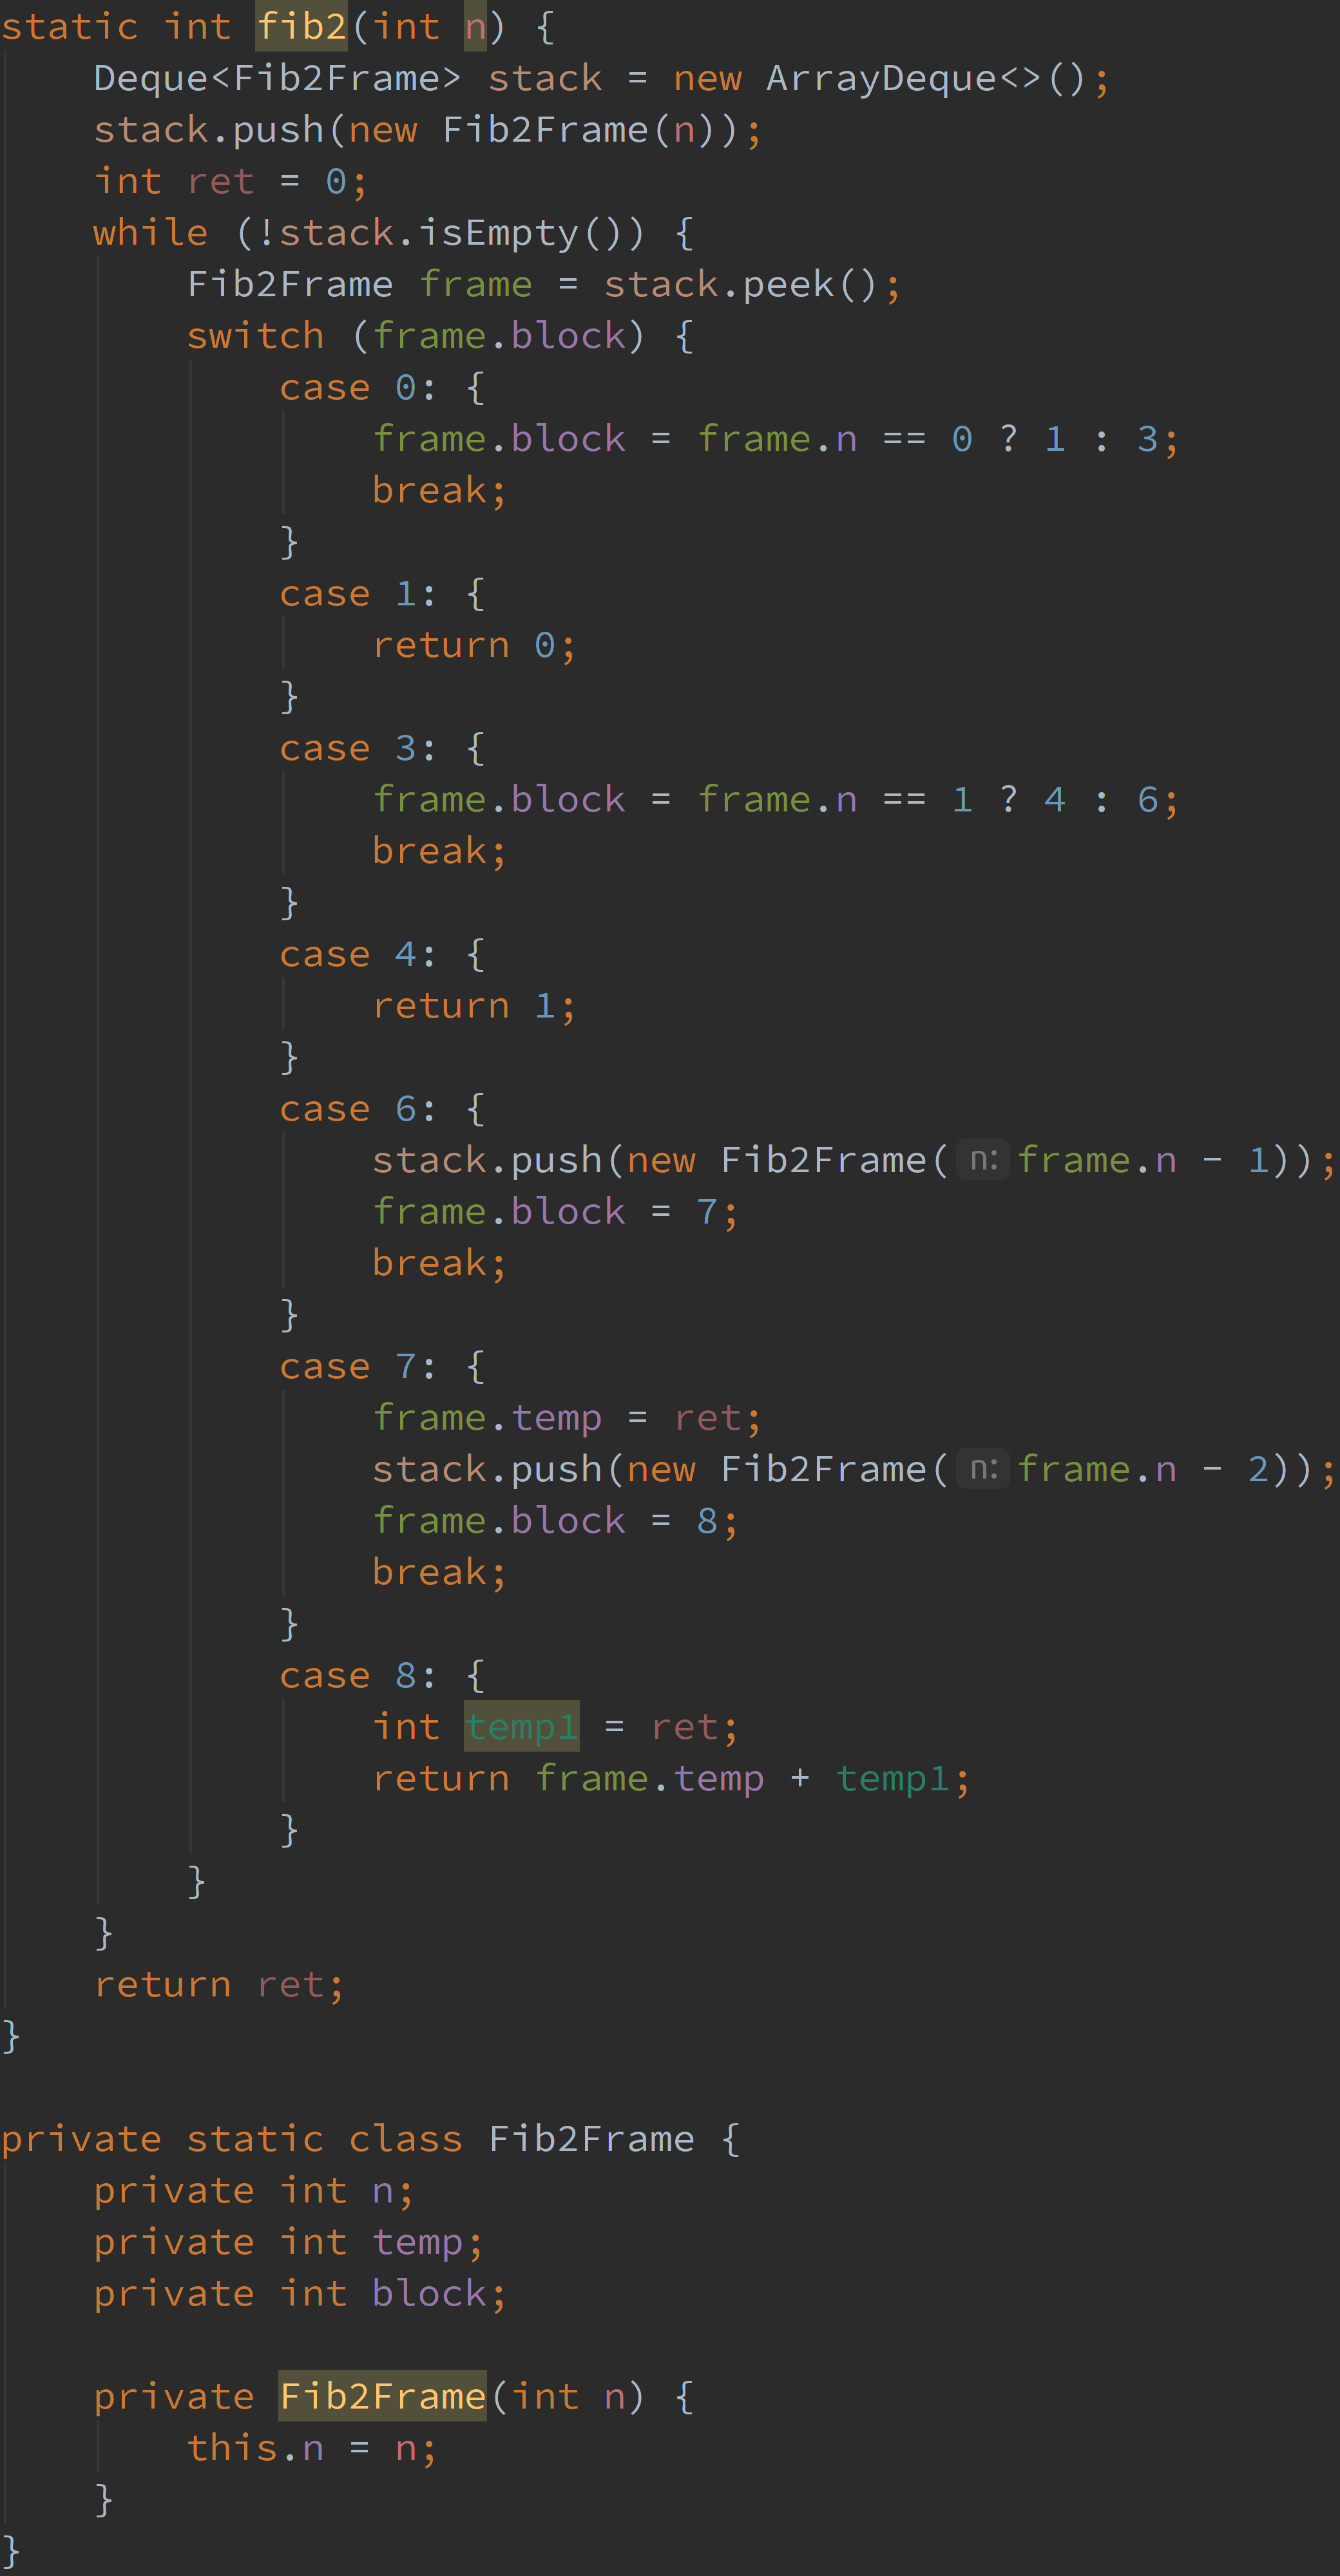
\includegraphics[height=4.464in]{src/img/remove-unreachable-after.png}
        \caption{After}
    \end{subfigure}%
    }\\
    \caption{Removing unreachable blocks \label{img:remove-unreachable}}
\end{figure}